\documentclass[./\jobname.tex]{subfiles}
\begin{document}
%
% The behavior of active/reactive classes shall be modeled using state chart diagrams where applicable.
% That means that for instance a TCP server, which is active/reactive does not need a state chart diagram.
% The state chart diagrams shall point out all states, transitions, events, actions and conditions.
% The use of a state event array is recommended.
%
\chapter{Verhaltensmodell}
%
In diesem Kapitel wird das Verhaltensmodell vorgestellt.
%
\section{Designmodelle}
%
Folgende Zustandsdiagramme beschreiben das Verhalten des Förderbandes im \modeA und \modeB.
Der Wechsel zwischen \modeA und \modeB ist nur im \enquote{Idle-State} erlaubt.\par
Bevor das Förderband im \modeB zum Pakettransport benutzt werden kann, bedarf es einer Betriebsmodiauswahl. Diese ist in  \autoref{fig: selectMode.pdf} dargestellt.
%
\begin{figure}[H]
	\centering
	\noindent\adjustbox{max width=\textwidth}{%falls größer als \textwidth, wird das Bild verkleinert
		%trim option's parameter order: left bottom right top
		\includegraphics[width=1\textwidth]{./img/3_verhaltensmodell/selectMode.pdf}
	}
	\unterschrift{Designmodell-Statemachine Choose Operating Mode}{Eigene Ausarbeitung}{}
	\label{fig: selectMode.pdf}
\end{figure}
%
Ist der Betriebsmodus \modeA angewählt, so wird die Statemachine in \autoref{fig: LocalMode.pdf} ausgeführt.
%
\begin{figure}[H]
	\centering
	\noindent\adjustbox{max width=\textwidth}{%falls größer als \textwidth, wird das Bild verkleinert
		%trim option's parameter order: left bottom right top
		\includegraphics[width=1\textwidth]{./img/3_verhaltensmodell/LocalMode.pdf}
	}
	\unterschrift{Designmodell-Substatemachine Locale Mode}{Eigene Ausarbeitung}{}
	\label{fig: LocalMode.pdf}
\end{figure}
%
Hingegen ist der Betriebsmodus \modeB angewählt, so wird die Statemachine in \autoref{fig: ChainMode.pdf} ausgeführt.
%
\begin{figure}[H]
	\centering
	\noindent\adjustbox{max width=\textwidth}{%falls größer als \textwidth, wird das Bild verkleinert
		%trim option's parameter order: left bottom right top
		\includegraphics[width=1\textwidth]{./img/3_verhaltensmodell/ChainMode.pdf}
	}
	\unterschrift{Designmodell-Substatemachine Chain Mode}{Eigene Ausarbeitung}{}
	\label{fig: ChainMode.pdf}
\end{figure}
%
Die Statemachines von \modeA und \modeB in den \cref{fig: ChainMode.pdf,fig: LocalMode.pdf} verwenden für den Zustand \enquote{Belt in motion} die Subsubstatemachine in \autoref{fig: BeltInMotion.pdf}.
%
\begin{figure}[H]
	\centering
	\noindent\adjustbox{max width=\textwidth}{%falls größer als \textwidth, wird das Bild verkleinert
		%trim option's parameter order: left bottom right top
		\includegraphics[width=1\textwidth]{./img/3_verhaltensmodell/BeltInMotion.pdf}
	}
	\unterschrift{Designmodell-Subsubstatemachine Drive Profile}{Eigene Ausarbeitung}{}
	\label{fig: BeltInMotion.pdf}
\end{figure}
%
\newpage
\section{Implementierungsmodelle}
\label{sec: Implementierungsmodelle}
%
In diesem Abschnitt wird die implementierte Statemachine erläutert. Dabei werden die Unterschiede zum Designmodell hervorgehoben. In den folgenden Diagrammen enthalten sind die Trigger (Events) und die Bedingungen, welche eine Transition zwischen zwei Zuständen auslöst sowie die Methode, die dabei aufgerufen wird, die in \autoref{sec: code statemachin} als Codeausschnitt eingesehen werden können. In \autoref{fig: implementation_selectMode.pdf} ist die Statemachine für die Betriebsmodiauswahl dargestellt. Im Vergleich zum Designmodell wurde der Zustand \enquote{startSystem} hinzugefügt.
%
\begin{figure}[H]
	\centering
	\noindent\adjustbox{max width=\textwidth}{%falls größer als \textwidth, wird das Bild verkleinert
		%trim option's parameter order: left bottom right top
		\includegraphics[width=1\textwidth]{./img/3_verhaltensmodell/implementation/selectMode.pdf}
	}
	\unterschrift{Implementierte-Statemachine Choose Operating Mode}{Eigene Ausarbeitung}{}
	\label{fig: implementation_selectMode.pdf}
\end{figure}
%
\newpage
Das Verhalten vom Local-Mode ist in \autoref{fig: implementation_LocalMode.pdf} dargestellt. Für die Initialisierung der Substatemachine wurde der Zustand \enquote{SelectLocalMode} hinzugefügt. Wird der Local-Mode Betriebsmodi gewählt, ändert sich der Zustand auf \enquote{Idle}. Im \enquote{Idle} Zustand kann wiederum auf den Chin-Mode gewechselt werden. Für das Erhöhen und Reduzieren der Maximalgeschwindigkeit wurde eine eigene Transition implementiert. Das selbe gilt für das Starten des Profils über die Richtungsauswahl links oder rechts.
%
\begin{figure}[H]
	\centering
	\noindent\adjustbox{max width=\textwidth}{%falls größer als \textwidth, wird das Bild verkleinert
		%trim option's parameter order: left bottom right top
		\includegraphics[width=1\textwidth]{./img/3_verhaltensmodell/implementation/LocalMode.pdf}
	}
	\unterschrift{Implementierte-Substatemachine Locale Mode}{Eigene Ausarbeitung}{}
	\label{fig: implementation_LocalMode.pdf}
\end{figure}
%
\newpage
In \autoref{fig: implementation_ChainMode.pdf} ist die implementierte Substatemachine, welche das Verhalten vom ChainMode repräsentiert, dargestellt. Im Vergleich zum Designmodell wurde der Zustand \enquote{SelectChainMode} für die Initialisierung hinzugefügt, der Zustand \enquote{Performing} durch eine Subsubstatemachine ersetzt und beim Zustand \enquote{Waiting} eine Abbruch-Transition hinzugefügt. Tritt aus unbekannten Gründen ein Fehler in der Paketübermittlung auf, kann mit dem \enquote{stop} Kommando bzw. mit der Keyboard Eingabe \enquote{c} der Chain-Mode resetet werden.
%
\begin{figure}[H]
	\centering
	\noindent\adjustbox{max width=\textwidth}{%falls größer als \textwidth, wird das Bild verkleinert
		%trim option's parameter order: left bottom right top
		\includegraphics[width=1\textwidth]{./img/3_verhaltensmodell/implementation/ChainMode.pdf}
	}
	\unterschrift{Implementierte-Substatemachine Chain Mode}{Eigene Ausarbeitung}{}
	\label{fig: implementation_ChainMode.pdf}
\end{figure}
%
\newpage
Die \autoref{fig: implementation_Performing.pdf} zeigt die neu hinzugefügte Subsubstatemachine \enquote{Performing}. Wird gerade ein Paket transportiert und erhält das Conveyor Belt einen \enquote{Request} wird die Methode \enquote{myAction41()} ausgeführt. Die Anfrage wird in einem Puffer gespeichert und sobald sich der \enquote{ChainMode} im Zustand \enquote{Idle} befindet, behandelt.
%
\begin{figure}[H]
	\centering
	\noindent\adjustbox{max width=\textwidth}{%falls größer als \textwidth, wird das Bild verkleinert
		%trim option's parameter order: left bottom right top
		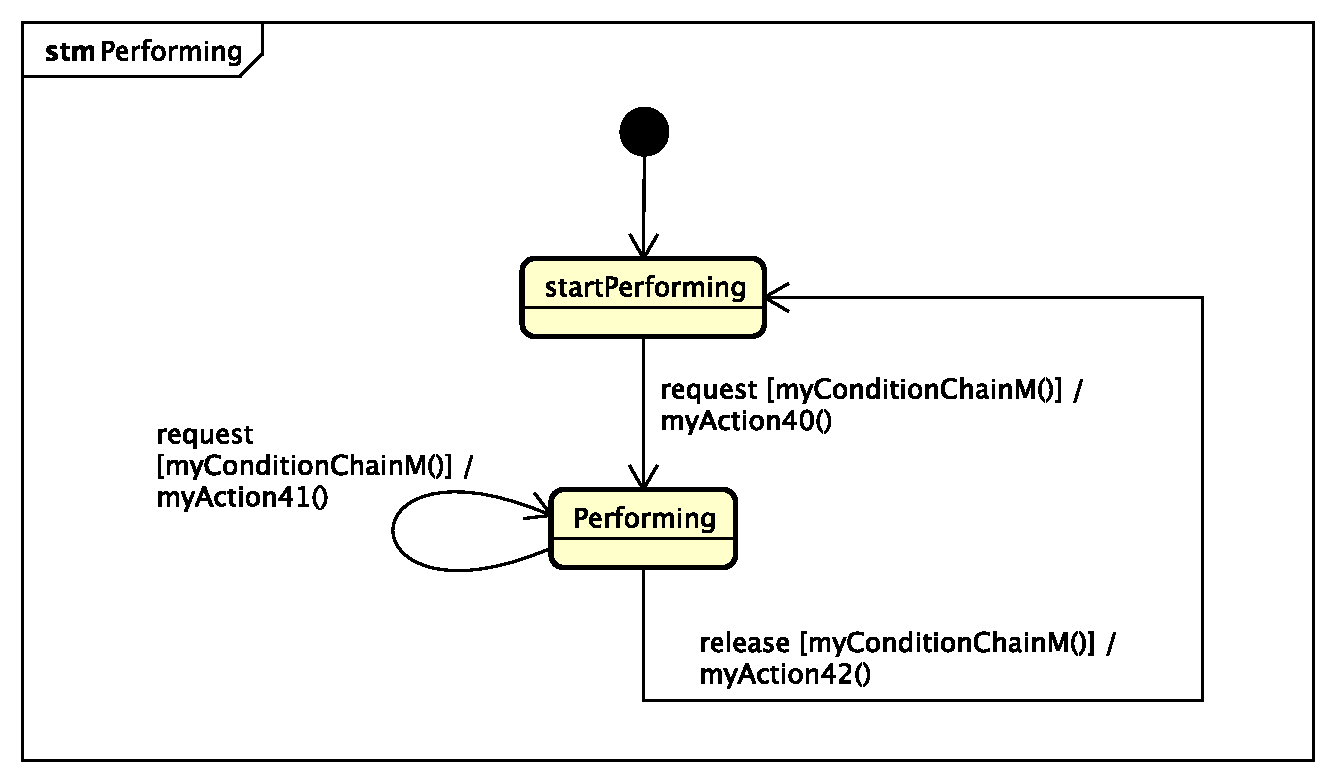
\includegraphics[width=1\textwidth]{./img/3_verhaltensmodell/implementation/Performing.pdf}
	}
	\unterschrift{Implementierte-Subsubstatemachine Performing}{Eigene Ausarbeitung}{}
	\label{fig: implementation_Performing.pdf}
\end{figure}
%
\newpage
Das Abfahren des Geschwindigkeitsprofils ist in \autoref{fig: implementation_BeltInMotion.pdf} dargestellt. Im Implementierungsmodell ist kein Timer wie im Designmodell enthalten. Dieser wird jetzt in der Klasse \enquote{Controller} implementiert.
\begin{figure}[H]
\centering
\noindent\adjustbox{max width=\textwidth}{%falls größer als \textwidth, wird das Bild verkleinert
	%trim option's parameter order: left bottom right top
	\includegraphics[width=1\textwidth]{./img/3_verhaltensmodell/implementation/BeltInMotion.pdf}
}
\unterschrift{Implementierte-Subsubstatemachine Drive Profile}{Eigene Ausarbeitung}{}
\label{fig: implementation_BeltInMotion.pdf}
\end{figure} 
%
\end{document}
